\chapter{Giải thuật quay lui}
\section{Giới thiệu}
Dùng để giải bài toán liệt kê cấu hình. Mỗi cấu hình được xây dựng bằng cách chọn từng phần tử, mỗi phần tử được chọn bằng cách thử tất cả các khả năng theo quy tắc nhân.

Mã giả cho thuật toán quay lui:
\begin{algorithmic}
    \State $x\gets[]$
    \Comment{Khai báo mảng $x$ lưu cấu hình hiện tại}
    \Function{Try}{$i$}
        \Comment{Thử cho phần tử $x_i$}
        \For{$j$ trong tập giá trị cho $x_i$}
            \State $x_i\gets j$
            \If{$i=n$}
                \Comment{$n$ là số phần tử của cấu hình}
                \State{Thông báo cấu hình trong $x$}
            \Else
                \State{<Thời điểm cuối cùng để ghi nhận kết quả>}
                \State\Call{Try}{i+1}
                \State{<Bỏ ghi nhận giá trị $x_i\gets j$ để thử giá trị khác>}
            \EndIf
        \EndFor
    \EndFunction
\end{algorithmic}

Thuật toán quay lui sẽ bắt đầu bằng lời gọi \texttt{Try(0)}, \texttt{Try(1)} hoặc với chỉ số mảng x mà ta muốn bắt đầu xây dựng.

Vì thuật toán này rất dễ nên tất cả các ví dụ trong bài này sẽ do người đọc tự làm.

\section{Liệt kê dãy nhị phân độ dài n}
Dùng mảng x để lưu dãy nhị phân hiện tại. Biết rằng $j\in\{0,1\}$.
\begin{figure}[h]
    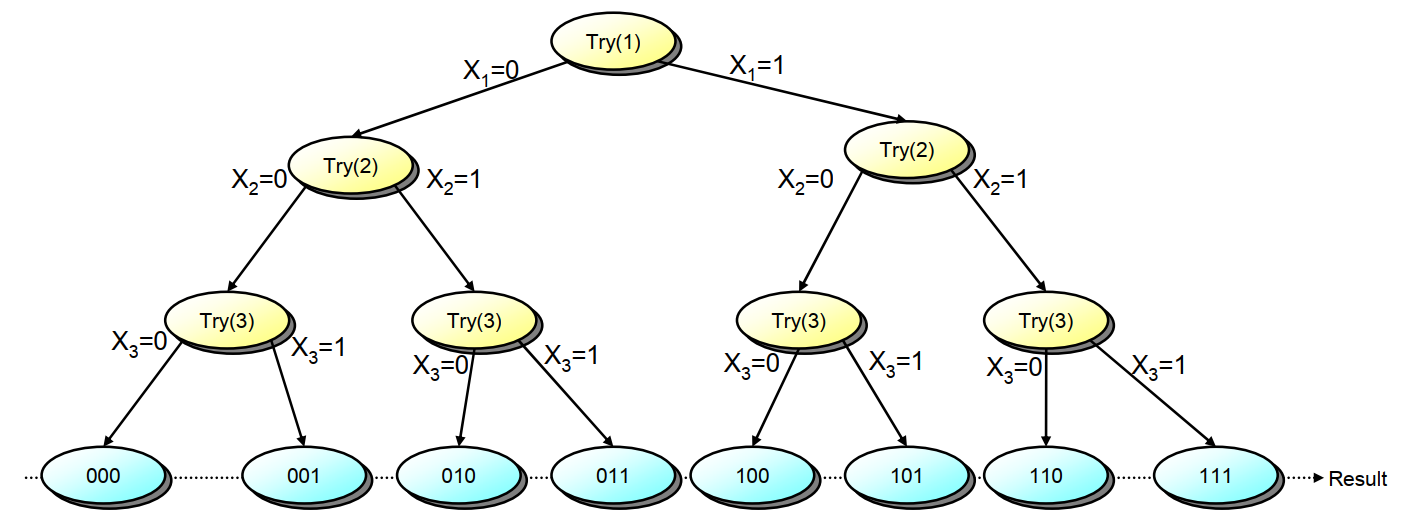
\includegraphics[scale=0.3]{quaylui/lknp.png}
    \caption{Cây tìm kiếm quay lui với n = 3}
\end{figure}

\section{Liệt kê các tổ hợp chập k}
Đây là bài toán biến thể của bài toán trên, với $j$ thuộc tập các phần tử (nếu nó chưa được chọn).

\section{Bài toán phân tích số}
Cho một số $n\leq30$, hãy liệt kê tất cả các cách phân tích nó thành một tổng.

\begin{tabular}{l|l}
    ANALYSE.INP & ANALYSE.OUT\cr\hline
    6 & 6 = 1 + 1 + 1 + 1 + 1 + 1\cr
      & 6 = 1 + 1 + 1 + 1 + 2\cr
      & 6 = 1 + 1 + 1 + 3\cr
      & 6 = 1 + 1 + 2 + 2\cr
      & 6 = 1 + 1 + 4\cr
      & 6 = 1 + 2 + 3\cr
      & 6 = 1 + 5\cr
      & 6 = 2 + 2 + 2\cr
      & 6 = 2 + 4\cr
      & 6 = 3 + 3\cr
      & 6 = 6\cr
\end{tabular}

Đây là bài toán biến thể của bài toán trên, với $j\in[1;n]$. Để cho thuận tiện ta dùng thêm mảng t với $t_i$ là tổng các phần tử từ $x_1\dots x_i$. Lưu ý:
\begin{itemize}
    \item Để tránh trùng lặp (hoán vị) ta sẽ đặt thêm điều kiện $x_i\geq x_{i-1}$.
    \item Để đặt điều kiện dừng (vì lần này ta không có số phần tử cố định) đồng thời tăng tốc độ cho đệ quy (không xét những giá trị thừa), ta chọn $x_i$ sao cho $t_{i+1}\leq n$ hay
    $$
        t_{i+1}\leq n\Leftrightarrow t_{i-1}+x_i+x_{i+1}\leq n\Leftrightarrow x_i+x_{i+1}\leq n-t_{i-1}
    $$
    mà $x_{i+1}\geq x_i$ nên suy ra $x_i\leq(n-t_{i-1})/2$. Ví dụ khi $n=10$ mà chọn $x_0\in\{6,7,8,9,10\}$ thì ta không thể chọn tiếp $x_1$, vậy chọn $x_0$ như vậy vô nghĩa.

    \textbf{Tóm lại: ta gọi đệ quy tìm tiếp khi $x_i$ được chọn còn cho phép chọn $x_{i+1}\geq x_i$ mà không làm tổng vượt quá n, ta in kết quả ở lần đệ quy cuối khi $t_i=n$.}
\end{itemize}

\section{Bài toán xếp hậu}
Cho bàn cờ vua n x n. Tìm cách xếp n quân hậu trên bàn cờ sao cho không quân nào ăn được quân nào.

Ví dụ n = 8:

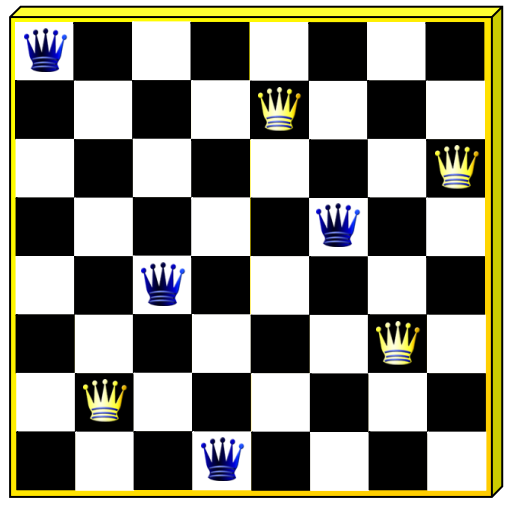
\includegraphics[scale=0.5]{quaylui/xephau.png}

Rõ ràng n quân hậu sẽ được đặt mỗi con 1 hàng vì hậu ăn ngang được, mỗi con 1 cột vì hậu cũng ăn dọc được, vậy nếu gọi quân hậu i là quân hậu ở hàng i, ta chỉ cần tìm ra vị trí cột của từng quân là sẽ giải được một nghiệm của bài toán. Có một tính chất dễ nhận thấy nếu ta làm các bài toán liên quan đến bảng nhiều:
\begin{itemize}
    \item Ta dùng mảng a để đánh dấu xem cột đó có con hậu nào chưa. ($a_i$ = true nếu đã có và ngược lại).
    \item Mọi đường chéo hướng ĐB-TN đều có các ô với số hàng + số cột là một hằng số C. 8 đường chéo có tổng lần lượt là 2, 4, \dots 2n. Vậy ta có thể dùng mảng b kích cỡ 2n với $a_C$ = true biểu thị đường chéo ĐB-TN chưa có quân hậu nào kiểm soát và ngược lại.
    \item Mọi đường chéo hướng ĐN-TB đều có các ô với số hàng - số cột là một hằng số C. Làm tương tự như trên với mảng c.
\end{itemize}

Vậy ta xây dựng thuật toán quay lui: Đặt từng quân hậu, đánh dấu trên các mảng a, b, c và gọi đệ quy đặt quân tiếp theo với điều kiện đã nêu $(a_j = b_{i+j} = c_{i-j}$ = true).